\newpage
\section{Addition $a+b$}

% ----------------------------------------------------------------------------
\subsection{Definition}

Die Addition ist eine Rechenoperation der ersten Stufe. Sie basiert auf dem Vorgang des Zusammenfassens von Dingen.

% ----------------------------------------------------------------------------
\subsection{Schreib- und Sprechweise}
Die beiden Zahlen $a$ und $b$, welche addiert werden, heissen \textbf{Summanden}, das Resultat $c$ heisst \textbf{Summe}.

Für die Addition wird das Operationszeichen $+$ verwendet. Wir schreiben
\[
  a + b = c
\]
und sagen «$a$ plus $b$ ist gleich $c$.» oder «Die Summe von $a$ und $b$ ist gleich $c$.»
\begin{example}
  \textbf{Beispiel:} Die Summe von Drei und Fünf ist gleich Acht: $3 + 5 = 8$
\end{example}

% ----------------------------------------------------------------------------
\subsection{Geometrische Interpretation}

Geometrisch gesehen ist eine Addition das aneinanderhängen zweier Längen.
\begin{center}
  \begin{tikzpicture}
    \tkzInit[xmin=0,xmax=9.5]
    \tkzDrawX[label={}]
    \tkzLabelX
    \tkzDefPoint(0,0){O}
    \tkzDefPoint(3,0){A}
    \tkzDefPoint(8,0){C}
    \tkzDrawSegment[dim={$3$,10pt,}](O,A)
    \tkzDrawSegment[dim={$5$,10pt,}](A,C)
    \tkzDrawSegment[dim={$8$,20pt,}](O,C)
  \end{tikzpicture}
\end{center}

So bedeutet $3+5$, dass die Distanz von $0$ zu $3$ und die Distanz von $0$ zu $5$ aneinandergehängt werden. Dabei wird der Punkt $8$ erreicht, also $3+5 = 8$.

% ----------------------------------------------------------------------------
\subsection{Kommutativgesetz}

Anhand der geometrischen Interpretation der Addition ist ersichtlich, dass es keine Rolle spielt, in welcher Reihenfolge die Summanden stehen. Wenn an die Länge $5$ die Länge $3$ angehängt wird, wird der gleiche Ort erreicht wie wenn an die Länge $3$ die Länge $5$ angehängt wird.
\begin{center}
  \begin{tikzpicture}
    \tkzInit[xmin=0,xmax=9.5]
    \tkzDrawX[label={}]
    \tkzLabelX
    \tkzDefPoint(0,0){O}
    \tkzDefPoint(3,0){A}
    \tkzDefPoint(5,0){B}
    \tkzDefPoint(8,0){C}
    \tkzDrawSegment[dim={$3$,10pt,}](O,A)
    \tkzDrawSegment[dim={$5$,10pt,}](A,C)
    \tkzDrawSegment[dim={$5$,20pt,}](O,B)
    \tkzDrawSegment[dim={$3$,20pt,}](B,C)
  \end{tikzpicture}
\end{center}
Diese Erkenntnis wird als mathematisches Gesetz formuliert:
\begin{theorem}
  \textbf{Kommutativgesetz.} Die Summanden einer Addition können vertauscht werden, ohne dass sich der Wert der Summe ändert.
  \[
    a + b = b + a
  \]
\end{theorem}

% ----------------------------------------------------------------------------
\subsection{Assoziativgesetz}

Grundsätzlich werden mehrere Additionen immer \textbf{von links nach rechts} ausgeführt. Um die Reihenfolge zu ändern, können Klammern verwendet werden. Operationen in Klammern werden zuerst ausgeführt.
\begin{example}
  \textbf{Beispiel:} Hier wird von links nach rechts gerechnet:
  \[
    2 + 3 + 4 = 5 + 4 = 9
  \]
  Hier wird zuerst die Addition in den Klammern ausgeführt:
  \[
    2 + (3 + 4) = 2 + 7 = 9
  \]
\end{example}

Offenbar spielt bei Addition diese Reihenfolge keine Rolle. Dies kann wieder anhand der geometrischen Darstellung auf der Zahlengerade gezeigt werden:
\begin{center}
  \begin{tikzpicture}
    \tkzInit[xmin=0,xmax=9.5]
    \tkzDrawX[label={}]
    \tkzLabelX
    \tkzDefPoint(0,0){O}
    \tkzDefPoint(2,0){A}
    \tkzDefPoint(5,0){B}
    \tkzDefPoint(9,0){C}
    \tkzDrawSegment[dim={$2$,12pt,}](O,A)
    \tkzDrawSegment[dim={$3+4$,12pt,}](A,C)
    \tkzDrawSegment[dim={$2+3$,24pt,}](O,B)
    \tkzDrawSegment[dim={$4$,24pt,}](B,C)
  \end{tikzpicture}
\end{center}
Auch diese Erkenntnis wird als mathematisches Gesetz formuliert:
\begin{theorem}
  \textbf{Assoziativgesetz.} Mehrere Additionen dürfen in beliebiger Reihenfolge ausgeführt werden, ohne dass sich der Wert der Summe ändert.
  \[
    a + b + c = (a + b) + c = a + (b + c)
  \]
\end{theorem}

% ----------------------------------------------------------------------------
\subsection{Neutralität der Null}

Die Zahl Null hat bezüglich der Addition eine besondere Stellung. Das Addieren von Null verändert den Wert nicht. Deshalb wird sie \textbf{neutral} bezüglich der Addition genannt.
\begin{theorem}
  \textbf{Neutralität der Null.} Zu einer Zahl kann Null addiert werden, ohne dass sich der Wert ändert:
  \[
    a + 0 = 0 + a = a
  \]
\end{theorem}
